% =====================================================================
%  Graph Autoencoders for Credit Card Fraud Detection
%  M.Sc. thesis-defense deck  --  Metropolis theme (conference quality)
%
%  Compile:
%     latexmk -pdf -shell-escape presentation.tex
%  or run twice with:  pdflatex / xelatex / lualatex
%  Dependencies: beamer, metropolis, tikz, pgfplots, booktabs
%
%  Speaker notes: \note{...} on each frame. To project them:
%     \setbeameroption{show notes on second screen=right}
%
%  All figures are vector TikZ/PGFPlots, factored into figures/*.tex
% =====================================================================
\documentclass[10pt,aspectratio=169]{beamer}

\usetheme{metropolis}
\usepackage{booktabs}
\usepackage{colortbl}
\usepackage{amsmath,amssymb}
\usepackage{tikz}
\usetikzlibrary{arrows.meta,positioning,calc}
\usepackage{pgfplots}
\pgfplotsset{compat=1.17}

% ---------------------------------------------------------------------
%  Deep Blue academic palette
% ---------------------------------------------------------------------
\definecolor{mDark}{HTML}{1F3A5F}    % Deep Navy  -- titles, dividers, networks
\definecolor{mBlue}{HTML}{4F81BD}    % Steel Blue -- secondary emphasis, entities, borders
\definecolor{mAccent}{HTML}{5DADE2}  % Sky Blue   -- highlights, arrows, markers, nodes
\definecolor{mGreen}{HTML}{27AE60}   % Green      -- gains / positive results
\definecolor{mOrange}{HTML}{F39C12}  % Orange     -- key numbers / best result (sparing)
\definecolor{mRed}{HTML}{C0392B}     % Muted Red  -- fraud / alerts / critique
\definecolor{mPurple}{HTML}{8E5BB5}  % Violet     -- emerging methods (lineage only)
\definecolor{mInk}{HTML}{222222}     % body text
% title-slide light text (on navy)
\definecolor{tSub}{HTML}{D6EAF8}     % subtitle
\definecolor{tSup}{HTML}{EAF2F8}     % supervisor
\definecolor{tFoot}{HTML}{D5DBDB}    % footer

\metroset{block=fill,sectionpage=none,numbering=fraction,progressbar=frametitle}

\setbeamercolor{normal text}{fg=mInk,bg=white}
\setbeamercolor{frametitle}{bg=mDark,fg=white}
\setbeamercolor{progress bar}{fg=mAccent,bg=mAccent!30}
\setbeamercolor{alerted text}{fg=mOrange}
\setbeamercolor{itemize item}{fg=mBlue}
\setbeamercolor{itemize subitem}{fg=mAccent}
\setbeamercolor{enumerate item}{fg=mDark}
% block palettes (Deep Navy title bar, light body)
\setbeamercolor{block title}{bg=mDark,fg=white}
\setbeamercolor{block body}{bg=mBlue!10,fg=mInk}
\setbeamercolor{block title alerted}{bg=mRed,fg=white}
\setbeamercolor{block body alerted}{bg=mRed!8,fg=mInk}
\setbeamercolor{block title example}{bg=mGreen,fg=white}
\setbeamercolor{block body example}{bg=mGreen!8,fg=mInk}
% title slide + closing standout
\setbeamercolor{title}{fg=mDark}
\setbeamercolor{subtitle}{fg=mBlue}
\setbeamercolor{author}{fg=mInk}
\setbeamercolor{institute}{fg=mInk}
\setbeamercolor{date}{fg=mInk}
\setbeamercolor{standout}{fg=white,bg=mDark}

% ---------------------------------------------------------------------
%  Reusable text + box macros (semantic colours)
% ---------------------------------------------------------------------
\newcommand{\hl}[1]{\textcolor{mBlue}{\textbf{#1}}}    % keyword highlight (steel)
\newcommand{\bl}[1]{\textcolor{mDark}{\textbf{#1}}}    % strong term (navy)
\newcommand{\gr}[1]{\textcolor{mGreen}{\textbf{#1}}}   % positive / gain
\newcommand{\rd}[1]{\textcolor{mRed}{\textbf{#1}}}     % fraud / alert / critique
\newcommand{\ob}[1]{\textcolor{mOrange}{\textbf{#1}}}  % key number / best (sparing)

\newenvironment{takeaway}{\begin{exampleblock}{Key takeaway}}{\end{exampleblock}}
\newenvironment{caveat}{\begin{alertblock}{Caveat}}{\end{alertblock}}

% ---------------------------------------------------------------------
%  Shared TikZ styles (inherited by every figures/*.tex)
% ---------------------------------------------------------------------
\tikzset{
  >=Stealth,
  cust/.style ={circle,fill=mBlue,text=white,align=center,inner sep=1pt,minimum size=0.95cm},
  merch/.style={circle,fill=mGreen,text=white,align=center,inner sep=1pt,minimum size=0.95cm},
  txn/.style  ={rectangle,rounded corners=2pt,fill=mDark,text=white,align=center,inner sep=2pt,minimum width=1.5cm,minimum height=0.9cm},
  stage/.style={rectangle,rounded corners=3pt,text=white,align=center,inner sep=3pt,minimum height=1.6cm},
  rel/.style  ={->,thick,mAccent},
}

% ---------------------------------------------------------------------
%  Custom section divider:  #1 number  #2 title  #3 one-line desc
% ---------------------------------------------------------------------
\newcommand{\sectionintro}[3]{%
  \begingroup
  \setbeamercolor{background canvas}{bg=mDark}
  \begin{frame}[plain]
    \vfill
    \begin{columns}[c]
      \begin{column}{0.92\textwidth}
        {\color{mAccent}\large\textbf{SECTION #1}}\par
        \vspace{6pt}
        {\color{white}\Huge\textbf{#2}}\par
        \vspace{12pt}
        {\color{mAccent}\rule{6cm}{1.4pt}}\par
        \vspace{12pt}
        {\color{white!80}\large #3}\par
      \end{column}
    \end{columns}
    \vfill
  \end{frame}
  \endgroup
}

% ---------------------------------------------------------------------
%  Outline row:  #1 number badge  #2 title  #3 short description
% ---------------------------------------------------------------------
\newcommand{\olrow}[3]{%
  \tikz[baseline=-0.7ex]{\node[fill=mDark,text=white,rounded corners=3pt,
        inner sep=0pt,minimum size=7.5mm,font=\bfseries]{#1};}%
  \hspace{0.6em}{\large\textbf{\textcolor{mDark}{#2}}}\hfill{\footnotesize\color{gray}#3}\par
  \vspace{0.45em}%
}

% ---------------------------------------------------------------------
%  Title metadata
% ---------------------------------------------------------------------
\title{Graph Autoencoders for Credit-Card Fraud Detection}
\subtitle{Unsupervised Learning on Graphs \& Heterogeneous Graph Auto-Encoders\\ A Critical Review}
\author{Luong Minh Duong \and Tran Le Phuong Thao \and Nguyen Nhu Thai}
\institute{Group 06 \quad\textbar\quad School of Information \& Communication Technology, HUST}
\date{Instructor: Prof.\ Nguyen Hung Son \quad\textbar\quad July 2026}

\IfFileExists{../Seminar_1/img/logo-soict-hust-1.png}
  {\titlegraphic{\hfill\includegraphics[height=1.25cm]{../Seminar_1/img/logo-soict-hust-1.png}}}
  {}

\begin{document}

% ===================== TITLE =====================
{% --- scoped Deep Navy background with faint transaction-network overlay ---
\setbeamercolor{background canvas}{bg=mDark}
\setbeamertemplate{background}{%
  \begin{tikzpicture}[remember picture,overlay]
    \fill[mDark] (current page.south west) rectangle (current page.north east);
    % faint network texture (top-right + bottom-left, away from the text)
    \begin{scope}[shift={(current page.center)},opacity=0.10]
      \foreach \a/\b/\c/\d in {%
          5.2/3.2/6.6/2.4, 5.2/3.2/4.6/1.8, 6.6/2.4/5.8/2.0,
          4.6/1.8/5.8/2.0, 6.6/2.4/6.9/3.6,
          -6.5/-3.2/-5.2/-2.4, -5.2/-2.4/-5.6/-2.0, -6.8/-1.8/-5.6/-2.0,
          -5.2/-2.4/-4.6/-3.4, -6.5/-3.2/-6.8/-1.8}
        \draw[white,line width=0.6pt] (\a,\b)--(\c,\d);
      \foreach \x/\y in {%
          5.2/3.2, 6.6/2.4, 4.6/1.8, 5.8/2.0, 6.9/3.6,
          -6.5/-3.2, -5.2/-2.4, -6.8/-1.8, -5.6/-2.0, -4.6/-3.4}
        \fill[white] (\x,\y) circle (2.4pt);
    \end{scope}
    \begin{scope}[shift={(current page.center)},opacity=0.18]
      \fill[mAccent] (5.8,2.0) circle (2.8pt);
      \fill[mAccent] (-5.6,-2.0) circle (2.8pt);
    \end{scope}
  \end{tikzpicture}%
}
\begin{frame}[plain]
  % --- Affiliation header + autoencoder glyph ---
  \begin{columns}[c,onlytextwidth]
    \begin{column}{0.80\textwidth}
      % {\color{white}\large\textbf{Hanoi University of Science and Technology}}\par
      % \vspace{1pt}
      % {\color{tSub}\small School of Information and Communication Technology}
    \end{column}
    \begin{column}{0.20\textwidth}
      \hfill
      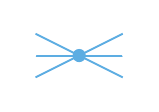
\begin{tikzpicture}[scale=0.30,>=Stealth,baseline]
        \foreach \y in {1,0,-1} \draw[mAccent,line width=0.7pt] (-2,\y)--(0,0);
        \foreach \y in {1,0,-1} \draw[mAccent,line width=0.7pt] (0,0)--(2,\y);
        \foreach \y in {1,0,-1} \fill[white] (-2,\y) circle (0.18);
        \foreach \y in {1,0,-1} \fill[white] (2,\y) circle (0.18);
        \fill[mAccent] (0,0) circle (0.28);
      \end{tikzpicture}
    \end{column}
  \end{columns}

  \vfill
  {\color{mAccent}\rule{\linewidth}{2pt}}\par
  \vspace{0.20cm}
  {\color{white}\fontsize{24}{29}\selectfont\bfseries
    Graph Autoencoders for\\ Credit-Card Fraud Detection\par}
  \vspace{0.16cm}
  {\color{tSub}\large Unsupervised learning on graphs and heterogeneous\\
    graph auto-encoders --- a critical review\par}
  \vfill

  % --- Authors + supervisor ---
  \begin{columns}[T,onlytextwidth]
    \begin{column}{0.58\textwidth}
      {\color{mAccent}\footnotesize\textbf{Group 6}}\par
      \vspace{3pt}
      {\color{white} Luong Minh Duong}~{\footnotesize\color{tSub}20251038M}\par
      {\color{white} Tran Le Phuong Thao}~{\footnotesize\color{tSub}20251186M}\par
      {\color{white} Nguyen Nhu Thai}~{\footnotesize\color{tSub}20252270M}\par
      \vspace{3pt}
      % {\color{tFoot}\footnotesize Seminar Group 06}
    \end{column}
    \begin{column}{0.40\textwidth}
      {\color{mAccent}\footnotesize\textbf{Supervisor}}\par
      \vspace{3pt}
      {\color{tSup} Prof.\ Nguyen Hung Son}\par
      \vspace{3pt}
      % {\color{tFoot}\footnotesize Dept.\ of Computer Science, SoICT}
    \end{column}
  \end{columns}

  \vfill
  {\color{mAccent}\rule{\linewidth}{0.6pt}}\par
  \vspace{2pt}
  % {\color{tFoot}\footnotesize M.Sc.\ Seminar \quad\textcolor{mOrange}{\textbullet}\quad Hanoi \quad\textcolor{mOrange}{\textbullet}\quad July 2026}
  % \vspace*{0.1cm}
\end{frame}
}
\note{Critical review of unsupervised graph learning for fraud detection; HGAE (Majumder 2025) as case study. Roadmap: motivation -> method -> evidence -> critique -> future. Q: "Your own model?" -> No; critique + agenda are our contribution.}

% ===================== OUTLINE =====================
\begin{frame}{Outline}
  \vspace{0.6em}
  \olrow{1}{Introduction}{Why credit-card fraud detection is hard}
  \olrow{2}{Background}{Graph-learning foundations for the model}
  \olrow{3}{Methodology}{How the HGAE works, step by step}
  \olrow{4}{Experiments}{Dataset, protocol, and metrics}
  \olrow{5}{Results}{What the numbers reveal --- read critically}
  \olrow{6}{Conclusion}{Takeaways and future directions}
\end{frame}
\note{30 s. Six acts. Promise the audience that by the end they will know what problem, why it matters, why graphs, how HGAE works, and what we found wrong.}

% =====================================================================
\section{Introduction}
% =====================================================================
\sectionintro{1}{Introduction}
  {Why detecting credit-card fraud is hard --- and why a label-free approach is needed.}
\note{Opening. We set the stage: fraud is rare and labels are scarce, so the whole talk is framed around a label-free, graph-based approach. Transition into the problem, the gap, and our objectives.}

% ---- Motivation ----
\begin{frame}{Fraud is rare --- and that is exactly the problem}
  \begin{columns}[T]
    \begin{column}{0.52\textwidth}
      \begin{itemize}
        \item Digital payments exploded $\rightarrow$ sophisticated fraud
        \item Supervised ML is the default defence\dots
        \item \dots but fraud labels are \rd{scarce, delayed, costly}
        \item Adversaries adapt $\rightarrow$ yesterday's labels age fast
      \end{itemize}
      \vspace{0.4em}
      \begin{takeaway}
        Learn what \hl{normal} looks like instead of chasing known fraud.
      \end{takeaway}
    \end{column}
    \begin{column}{0.46\textwidth}
      \centering
      \vspace{1.2em}
      % Class-imbalance pie chart (true proportions: the tiny fraud sliver IS the point)
\resizebox{\linewidth}{!}{%
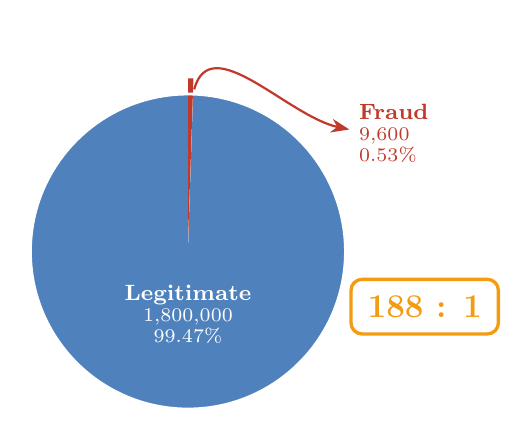
\begin{tikzpicture}[font=\footnotesize,>=Stealth]
  \def\R{2}
  % Legitimate slice (steel) -- 99.47%, sweeps 358.1 deg clockwise from 88.1 to -270
  \fill[mBlue] (0,0) -- (88.1:\R) arc[start angle=88.1, end angle=-270, radius=\R] -- cycle;
  % Fraud slice (red) -- 0.53% (~1.9 deg), slightly exploded along its bisector
  \begin{scope}[shift={(89.05:0.20)}]
    \fill[mRed] (0,0) -- (90:\R) arc[start angle=90, end angle=88.1, radius=\R] -- cycle;
  \end{scope}
  \draw[white,line width=1pt] (0,0) circle (\R);

  % Legitimate label (inside)
  \node[white,align=center] at (0,-0.8)
        {\textbf{Legitimate}\\[-2pt]\scriptsize 1{,}800{,}000\\[-2pt]\scriptsize 99.47\%};

  % Fraud leader + label
  \draw[mRed,thick,->] (0.08,\R+0.06) to[out=75,in=168] (2.05,1.55);
  \node[anchor=west,mRed,align=left] at (2.05,1.5)
        {\textbf{Fraud}\\[-2pt]\scriptsize 9{,}600\\[-2pt]\scriptsize 0.53\%};

  % Imbalance ratio (key number -> orange)
  \node[anchor=west,draw=mOrange,line width=1.2pt,rounded corners=4pt,inner sep=6pt,
        text=mOrange,font=\large\bfseries] at (2.05,-0.7) {188 : 1};
\end{tikzpicture}%
}

    \end{column}
  \end{columns}
\end{frame}
\note{1.5 min. Donut/bar: 1.8M vs 9.6K. Q: "Why not collect more labels?" -> arrive weeks later via chargebacks; adversaries shift meanwhile.}

% ---- Problem statement ----
\begin{frame}{Problem: extreme imbalance meets relational data}
  \begin{columns}[T]
    \begin{column}{0.5\textwidth}
      \begin{itemize}
        \item \rd{188 : 1} imbalance breaks supervised training
        \item Resampling (SMOTE) $\rightarrow$ \hl{overfitting} / lost structure
        \item Transactions are \bl{relational}, not i.i.d.\ rows
      \end{itemize}
    \end{column}
    \begin{column}{0.5\textwidth}
      \begin{block}{Research question}
        Can we detect fraud \emph{without fraud labels} by learning the \hl{topology} and \hl{attributes} of legitimate behaviour?
      \end{block}
    \end{column}
  \end{columns}
\end{frame}
\note{1 min. The block is the thesis of the whole talk. Q: "Isn't anomaly detection standard?" -> yes, but on a type-aware heterogeneous graph is the angle.}

% ---- Research gap ----
\begin{frame}{Why existing methods fall short}
  \begin{columns}[T]
    \begin{column}{0.5\textwidth}
      \textbf{Supervised / tabular}
      \begin{itemize}
        \item Need many labels $\rightarrow$ infeasible
        \item Treat each transaction as \rd{isolated}
        \item Ignore shared cards / merchants / bursts
      \end{itemize}
    \end{column}
    \begin{column}{0.5\textwidth}
      \textbf{What we actually need}
      \begin{itemize}
        \item Works with \gr{few / no labels}
        \item Captures \gr{relational} structure
        \item Stays \gr{scalable} \& \gr{interpretable}
      \end{itemize}
    \end{column}
  \end{columns}
  \vspace{0.3em}
  \begin{takeaway}
    Topology is precisely the signal row-wise classifiers discard.
  \end{takeaway}
\end{frame}
\note{1 min. The gap motivates graphs + unsupervised. Bridge to objectives.}

% ---- Objectives ----
\begin{frame}{Objectives \& contributions}
  \begin{enumerate}
    \item \hl{Survey}: from message-passing GNNs to self-supervised GAEs
    \item \hl{Dissect}: the Heterogeneous Graph Auto-Encoder (HGAE)
    \item \hl{Evaluate}: architecture, training, reported results --- critically
    \item \rd{Expose}: formulation \& reproducibility gaps \quad\textit{(our contribution)}
    \item \rd{Propose}: research agenda for robust detection \quad\textit{(our contribution)}
  \end{enumerate}
\end{frame}
\note{1 min. Stress: items 4-5 are original. Q: "Novelty?" -> the critique and the agenda.}

% =====================================================================
\section{Background}
% =====================================================================
\sectionintro{2}{Background}
  {The graph-learning foundations needed to understand the model.}
\note{Bridge: We have established WHY the problem matters and WHAT we aim to do. Before the method we need a shared vocabulary --- message passing, attention, and the auto-encoder principle. That is this section.}

% ---- Lineage ----
\begin{frame}{HGAE stands on two intellectual lines}
  \centering
  % Evolution / lineage timeline of graph representation learning
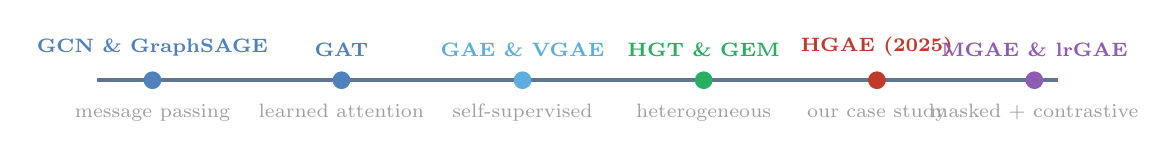
\begin{tikzpicture}[font=\scriptsize]
  \draw[line width=1.6pt,mDark!70] (0,0) -- (12.2,0);
  \foreach \x/\c/\t/\b in {%
      0.7/mBlue/{GCN \& GraphSAGE}/{message passing},
      3.1/mBlue/{GAT}/{learned attention},
      5.4/mAccent/{GAE \& VGAE}/{self-supervised},
      7.7/mGreen/{HGT \& GEM}/{heterogeneous},
      9.9/mRed/{\textbf{HGAE} (2025)}/{our case study},
      11.9/mPurple/{MGAE \& lrGAE}/{masked + contrastive}}{%
    \fill[\c] (\x,0) circle (3.2pt);
    \node[\c,align=center,anchor=south] at (\x,0.18) {\textbf{\t}};
    \node[gray!75,align=center,anchor=north] at (\x,-0.18) {\b};
  }
\end{tikzpicture}

  \vfill
  \begin{columns}[T]
    \begin{column}{0.5\textwidth}
      \footnotesize \bl{Heterogeneous attention}\\ HGT, GEM --- type/relation-aware
    \end{column}
    \begin{column}{0.5\textwidth}
      \footnotesize \hl{Reconstruction self-supervision}\\ GAE, VGAE --- no labels
    \end{column}
  \end{columns}
\end{frame}
\note{1.5 min. Red node = case study; purple previews future work. Q: "vs GEM?" -> GEM semi-supervised over accounts/devices; HGAE unsupervised attribute reconstruction.}

% ---- Message passing + key limits ----
\begin{frame}{Background: message passing, attention, and its limits}
  \begin{itemize}
    \item \textbf{Message passing}: a node refines itself by aggregating neighbours
    \item \textbf{GAT}: learns \emph{how much} each neighbour matters
    \item \textbf{Permutation equivariance}: the right inductive bias for networks
  \end{itemize}
  \vspace{0.3em}
  \begin{caveat}
    Power bounded by the \rd{1-WL} test; deep stacks cause \rd{oversmoothing}.
    \textit{(Both return in our critique.)}
  \end{caveat}
\end{frame}
\note{1.5 min. Honesty up front builds credibility. Q: "engineer aggregate features?" -> loses learned multi-hop type-aware aggregation.}

% ---- GAE principle ----
\begin{frame}{The core idea: reconstruction error as an anomaly score}
  \begin{columns}[T]
    \begin{column}{0.55\textwidth}
      \begin{itemize}
        \item Encoder compresses graph $\rightarrow$ latent $Z$
        \item Decoder reconstructs the input
        \item Train on \gr{normal} data only
        \item Anomalies $\rightarrow$ \rd{high reconstruction error}
      \end{itemize}
    \end{column}
    \begin{column}{0.45\textwidth}
      \begin{block}{One-class framing}
        Never having modelled fraud, the decoder rebuilds it \emph{poorly} --- the error betrays it.
      \end{block}
    \end{column}
  \end{columns}
\end{frame}
\note{1 min. This principle is the conceptual core HGAE adapts. Sets up the whole method section.}

% =====================================================================
\section{Methodology}
% =====================================================================
\sectionintro{3}{Methodology}
  {How the Heterogeneous Graph Auto-Encoder turns transactions into anomaly scores.}
\note{Bridge: With the background in place --- GNNs aggregate neighbours, and auto-encoders flag anomalies via reconstruction error --- we can now assemble the actual model, built up step by step.}

% ---- Graph construction ----
\begin{frame}{Step 1 --- Lift transactions into a heterogeneous graph}
  \centering
  % Heterogeneous transaction graph construction
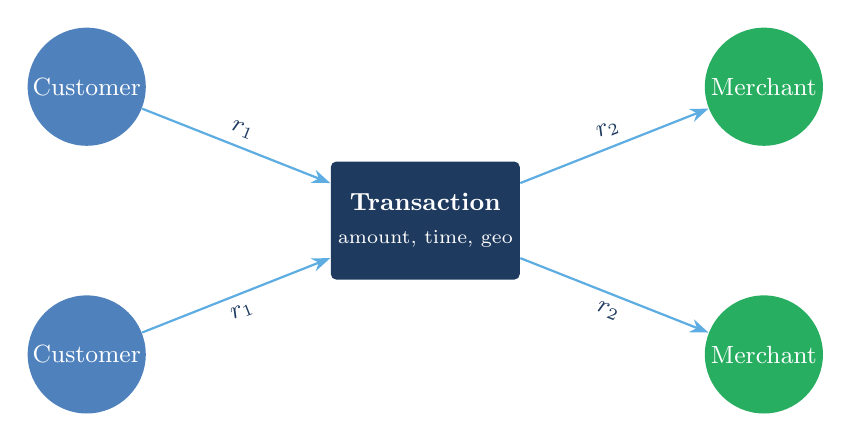
\begin{tikzpicture}[font=\normalsize,>=Stealth,
    cbig/.style={cust,minimum size=1.5cm,font=\small},
    mbig/.style={merch,minimum size=1.5cm,font=\small}]
  \node[cbig]  (c1) at (0,1.7)  {Customer};
  \node[cbig]  (c2) at (0,-1.7) {Customer};
  \node[txn,minimum width=2.4cm,minimum height=1.5cm,font=\small] (t) at (4.3,0)
        {\textbf{Transaction}\\[1pt]\scriptsize amount, time, geo};
  \node[mbig] (m1) at (8.6,1.7) {Merchant};
  \node[mbig] (m2) at (8.6,-1.7){Merchant};

  \draw[rel] (c1) -- node[above,sloped,mDark,font=\small]{$r_1$} (t);
  \draw[rel] (c2) -- node[below,sloped,mDark,font=\small]{$r_1$} (t);
  \draw[rel] (t) -- node[above,sloped,mDark,font=\small]{$r_2$} (m1);
  \draw[rel] (t) -- node[below,sloped,mDark,font=\small]{$r_2$} (m2);
\end{tikzpicture}

  \vspace{0.6em}
  \begin{columns}[T]
    \begin{column}{0.5\textwidth}
      \footnotesize \textbf{Three node types}, typed edges $r_1,r_2$
    \end{column}
    \begin{column}{0.5\textwidth}
      \footnotesize IDs $\to$ connectivity only (not features)\\ \rd{is\_fraud excluded from training}
    \end{column}
  \end{columns}
\end{frame}
\note{2 min. The is\_fraud exclusion is what makes it unsupervised. Q: "why IDs not features?" -> no metric meaning; leakage risk.}

% ---- Feature encoding ----
\begin{frame}{Step 2 --- Encode attributes into a shared space}
  \begin{itemize}
    \item Continuous (amount, time, geo) $\rightarrow$ \bl{standardised}
    \item Categorical (gender, category) $\rightarrow$ \bl{one-hot}
    \item Missing $\rightarrow$ per-type \bl{mean / mode}
    \item Concatenate $\Rightarrow$ layer-0 input $h^0$
  \end{itemize}
  \vspace{0.2em}
  \begin{block}{}
    Three types $\Rightarrow$ different dimensions $\Rightarrow$ reconciled by \hl{type-specific linear projections}.
  \end{block}
\end{frame}
\note{1 min. Bridges to the encoder. Q: "heterogeneous sizes?" -> each type its own projection into common dim.}

% ---- Architecture overview (built up with overlays) ----
\begin{frame}{Step 3 --- The HGAE pipeline at a glance}
  \centering
  % HGAE encoder -> latent -> decoder -> anomaly score pipeline
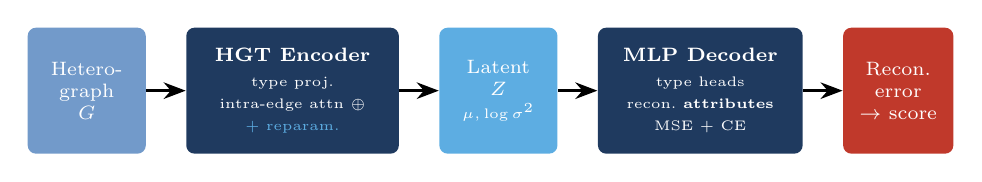
\begin{tikzpicture}[font=\scriptsize,>=Stealth,node distance=5mm]
  \node[stage,fill=mBlue!80,minimum width=1.5cm] (g)
        {Hetero-\\graph\\$G$};
  \node[stage,fill=mDark,minimum width=2.7cm,right=of g] (e)
        {\textbf{HGT Encoder}\\[1pt]\tiny type proj.\\\tiny intra-edge attn $\oplus$\\\tiny \textcolor{mAccent}{+ reparam.}};
  \node[stage,fill=mAccent,minimum width=1.5cm,right=of e] (z)
        {Latent\\$Z$\\\tiny $\mu,\log\sigma^2$};
  \node[stage,fill=mDark,minimum width=2.6cm,right=of z] (d)
        {\textbf{MLP Decoder}\\[1pt]\tiny type heads\\\tiny recon.\ \textbf{attributes}\\\tiny MSE + CE};
  \node[stage,fill=mRed,minimum width=1.4cm,right=of d] (s)
        {Recon.\\error\\$\to$ score};

  \draw[->,line width=1.1pt] (g)--(e);
  \draw[->,line width=1.1pt] (e)--(z);
  \draw[->,line width=1.1pt] (z)--(d);
  \draw[->,line width=1.1pt] (d)--(s);
\end{tikzpicture}

  \vspace{0.6em}
  \begin{itemize}\footnotesize
    \item<2-> \bl{Encoder} (HGT): type projections + intra-edge attention + reparameterization
    \item<3-> \hl{Latent $Z$}: a smooth, probabilistic embedding space
    \item<4-> \textbf{Decoder} reconstructs \rd{attributes}, \emph{not} adjacency $\rightarrow$ error = score
  \end{itemize}
\end{frame}
\note{2 min. Reveal one stage at a time. Stress attribute (not adjacency) reconstruction -- a key criticism later. Complexity ~ O(nE).}

% ---- Intra-edge attention (the novelty) ----
\begin{frame}{Key novelty --- intra-edge attention respects entity types}
  \centering
  % Standard GAT vs HGAE intra-edge attention (two-panel comparison)
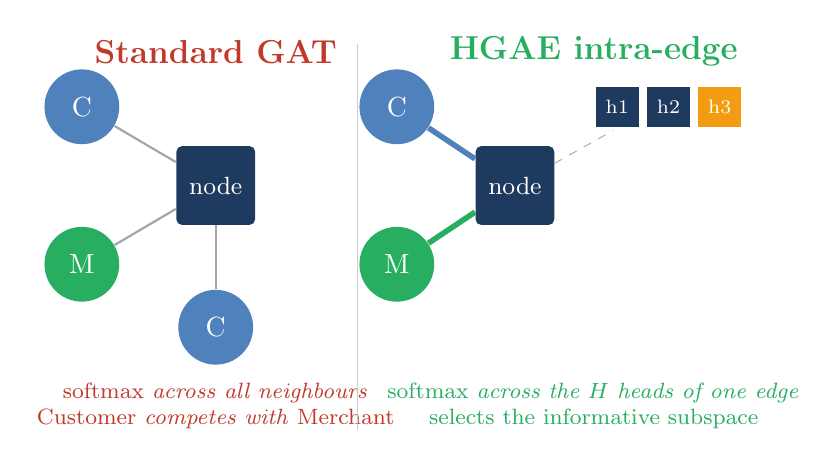
\begin{tikzpicture}[font=\small,>=Stealth]
  % ---- LEFT: GAT ----
  \node[mRed,font=\large\bfseries] at (1.9,3.1) {Standard GAT};
  \node[txn,minimum width=1.0cm,minimum height=1.0cm,font=\small] (n) at (1.9,1.4) {node};
  \node[cust,minimum size=0.95cm,font=\normalsize] (a) at (0.2,2.4) {C};
  \node[merch,minimum size=0.95cm,font=\normalsize] (b) at (0.2,0.4) {M};
  \node[cust,minimum size=0.95cm,font=\normalsize] (cc) at (1.9,-0.4) {C};
  \draw[gray!70,thick] (a)--(n); \draw[gray!70,thick] (b)--(n); \draw[gray!70,thick] (cc)--(n);
  \node[mRed,align=center,font=\footnotesize] at (1.9,-1.4)
        {softmax \emph{across all neighbours}\\Customer \emph{competes with} Merchant};

  % divider
  \draw[gray!40] (3.7,-1.7) -- (3.7,3.2);

  % ---- RIGHT: HGAE ----
  \node[mGreen,font=\large\bfseries] at (6.7,3.1) {HGAE intra-edge};
  \node[txn,minimum width=1.0cm,minimum height=1.0cm,font=\small] (n2) at (5.7,1.4) {node};
  \node[cust,minimum size=0.95cm,font=\normalsize] (a2) at (4.2,2.4) {C};
  \node[merch,minimum size=0.95cm,font=\normalsize] (b2) at (4.2,0.4) {M};
  \draw[mBlue,line width=2pt] (a2)--(n2);
  \draw[mGreen,line width=2pt] (b2)--(n2);
  % heads
  \node[draw=mDark,fill=mDark,text=white,font=\scriptsize,minimum size=5mm] (h1) at (7.0,2.4) {h1};
  \node[draw=mDark,fill=mDark,text=white,font=\scriptsize,minimum size=5mm] (h2) at (7.65,2.4) {h2};
  \node[draw=mOrange,fill=mOrange,text=white,font=\scriptsize,minimum size=5mm] (h3) at (8.3,2.4) {h3};
  \draw[gray!60,dashed] (n2) -- (6.95,2.1);
  \node[mGreen,align=center,font=\footnotesize] at (6.7,-1.4)
        {softmax \emph{across the $H$ heads of one edge}\\selects the informative subspace};
\end{tikzpicture}
\\[0.4em]
  {\footnotesize $f_{\text{Attent}}=\mathrm{Softmax}\!\big(\,\|_{k\in[1,H]}\mathrm{Att}^k(v_t,e_r,d_t)\big)$ \;---\; normalised over \gr{heads}, not neighbours}
\end{frame}
\note{2 min. GAT forces types to compete; HGAE selects the informative subspace per edge, preserving message magnitude (element-wise add). Each relation owns W\_Att, W\_Mssg.}

% ---- Latent space ----
\begin{frame}{Step 4 --- A probabilistic latent space}
  \begin{columns}[T]
    \begin{column}{0.55\textwidth}
      \begin{itemize}
        \item Reparameterization at the final encoder layer
        \item Each embedding $=$ a \bl{Gaussian} (mean, log-var)
        \item Noise $\rightarrow$ \gr{smooth} space; sampling stays \hl{differentiable}
      \end{itemize}
      \[ h = \text{mean}(h) + \epsilon\cdot\exp\!\big(\tfrac12\log(h)\big),\quad \epsilon\sim\mathcal N(0,1) \]
    \end{column}
    \begin{column}{0.45\textwidth}
      \begin{caveat}
        Loss has \rd{no KL term} $\Rightarrow$ strictly a noise-injected AE, not a true VAE.
      \end{caveat}
    \end{column}
  \end{columns}
\end{frame}
\note{1.5 min. Flag the caveat now so the later critique pays off. Q: "really variational?" -> no, without KL.}

% ---- Decoder + threshold ----
\begin{frame}{Step 5 --- Decode, then threshold the error}
  \begin{columns}[T]
    \begin{column}{0.40\textwidth}
      \begin{itemize}\footnotesize
        \item Type-specific MLP decoder
        \item err below $\tau$ $\Rightarrow$ \gr{Non-Fraud}
        \item err above $\tau$ $\Rightarrow$ \rd{Fraud}
      \end{itemize}
      \[\tau=\mu+2\sigma\]
      {\scriptsize $\approx 95\%$ interval of normal error}
    \end{column}
    \begin{column}{0.60\textwidth}
      \centering
      % Reconstruction-error distributions with anomaly threshold
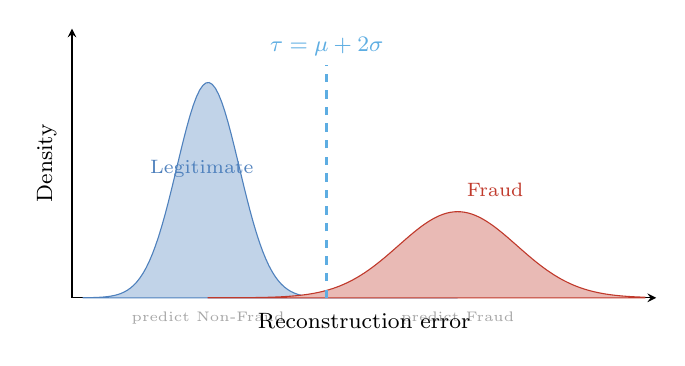
\begin{tikzpicture}
  \begin{axis}[
      width=9cm,height=5cm,
      axis lines=left,
      xlabel={\footnotesize Reconstruction error},
      ylabel={\footnotesize Density},
      xtick=\empty,ytick=\empty,
      ymin=0,ymax=1.25,clip=false,
      enlarge x limits=0.02]
    \addplot[draw=mBlue,fill=mBlue!35,domain=0:6,samples=120]{exp(-(x-2)^2/0.5)} \closedcycle;
    \addplot[draw=mRed,fill=mRed!35,domain=2:9,samples=120]{0.4*exp(-(x-6)^2/1.8)} \closedcycle;
    \draw[mAccent,very thick,dashed] (axis cs:3.9,0) -- (axis cs:3.9,1.08);
    \node[mAccent,anchor=south,font=\footnotesize\bfseries] at (axis cs:3.9,1.08) {$\tau=\mu+2\sigma$};
    \node[mBlue,font=\scriptsize] at (axis cs:1.9,0.6) {Legitimate};
    \node[mRed,font=\scriptsize] at (axis cs:6.6,0.5) {Fraud};
    \node[gray!70,font=\tiny,anchor=north] at (axis cs:2.0,-0.02) {predict Non-Fraud};
    \node[gray!70,font=\tiny,anchor=north] at (axis cs:6.0,-0.02) {predict Fraud};
  \end{axis}
\end{tikzpicture}

    \end{column}
  \end{columns}
\end{frame}
\note{1.5 min. Fraud is out-of-distribution -> error spikes right of tau. The Gaussian assumption is fragile (future work).}

% ---- Training pipeline + loss ----
\begin{frame}{Step 6 --- Three-phase training, no fraud labels in the loss}
  \centering
  % Three-phase train / calibrate / infer pipeline
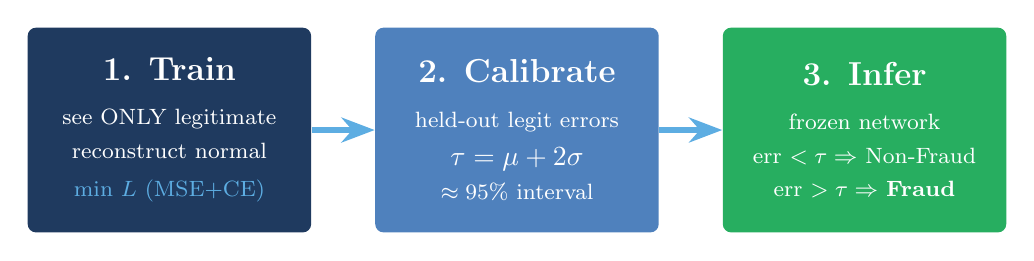
\begin{tikzpicture}[font=\normalsize,>=Stealth,node distance=8mm]
  \node[stage,fill=mDark,minimum width=3.6cm,minimum height=2.6cm] (p1)
        {\large\textbf{1. Train}\\[4pt]\footnotesize see ONLY legitimate\\\footnotesize reconstruct normal\\[2pt]\textcolor{mAccent}{\footnotesize min $L$ (MSE+CE)}};
  \node[stage,fill=mBlue,minimum width=3.6cm,minimum height=2.6cm,right=of p1] (p2)
        {\large\textbf{2. Calibrate}\\[4pt]\footnotesize held-out legit errors\\[2pt]\normalsize$\tau=\mu+2\sigma$\\\footnotesize $\approx 95\%$ interval};
  \node[stage,fill=mGreen,minimum width=3.6cm,minimum height=2.6cm,right=of p2] (p3)
        {\large\textbf{3. Infer}\\[4pt]\footnotesize frozen network\\\footnotesize err $<\tau\Rightarrow$ Non-Fraud\\\footnotesize err $>\tau\Rightarrow$ \textbf{Fraud}};
  \draw[->,line width=2pt,mAccent] (p1)--(p2);
  \draw[->,line width=2pt,mAccent] (p2)--(p3);
\end{tikzpicture}

  \vspace{0.5em}
  \[ L=\sum_{\forall N}\sum_{\forall t}\mathrm{LOSS}(d_t,d'_t) \]
  {\footnotesize \bl{MSE} for continuous attributes \;$+$\; \bl{CE} for categorical attributes}
\end{frame}
\note{1.5 min. Labels only calibrate + evaluate. No KL term (again). O(nE) foreshadows scalability limit. Q: "guarantee clean train data?" -> historically-cleared txns; contamination is a risk.}

% =====================================================================
\section{Experiments}
% =====================================================================
\sectionintro{4}{Experiments}
  {The dataset, protocol, and metrics used to put the model to the test.}
\note{Bridge: We now understand HOW the model works end to end. The natural next question is whether it actually works --- so we turn to the data, the protocol, and the right metrics.}

% ---- Dataset ----
\begin{frame}{Dataset --- a realistic, highly imbalanced log}
  \centering
  \begin{tabular}{ll}
    \arrayrulecolor{mDark}\toprule
    \rowcolor{mDark}\textcolor{white}{\textbf{Property}} & \textcolor{white}{\textbf{Value}}\\
    \midrule
    \rowcolor{mBlue!8} Total transactions & $\sim$1{,}809{,}600\\
    Fraudulent & $\sim$9{,}600 \;(\rd{$\approx$0.53\%})\\
    \rowcolor{mBlue!8} Node types & Customer, Merchant, Transaction\\
    Key fields & cc\_num, merchant\_id, amount, time, geo\\
    \rowcolor{mBlue!8} Label usage & \hl{calibration \& evaluation only}\\
    \bottomrule
  \end{tabular}
\end{frame}
\note{1 min. The 0.53\% positive rate defines the problem. Q: "public benchmark?" -> mirrors simulated CC-fraud datasets; figures from Majumder et al.}

% ---- Setup + metrics ----
\begin{frame}{Setup \& why AUC-PR is the metric that matters}
  \begin{columns}[T]
    \begin{column}{0.5\textwidth}
      \textbf{Setup}
      \begin{itemize}\footnotesize
        \item Train on \gr{legitimate-only} split
        \item Calibrate $\tau$ on held-out legit
        \item Baselines: \bl{GraphSAGE}, \bl{FI-GRL}
      \end{itemize}
    \end{column}
    \begin{column}{0.5\textwidth}
      \textbf{Metrics}
      \begin{itemize}\footnotesize
        \item \hl{AUC-PR} --- key under imbalance
        \item \hl{F1} --- precision/recall at $\tau$
        \item ROC-AUC --- \rd{optimistic} when negatives dominate
      \end{itemize}
    \end{column}
  \end{columns}
  \vspace{0.2em}
  \begin{caveat}
    Reported encoder depth \rd{= 124 layers} --- implausible under oversmoothing; blocks reproduction.
  \end{caveat}
\end{frame}
\note{1.5 min. With 0.53\% positives, accuracy is useless (99.5\% trivially). Surface the 124-layer flag.}

% =====================================================================
\section{Results}
% =====================================================================
\sectionintro{5}{Results}
  {What the numbers reveal --- and a critical reading of their limits.}
\note{Bridge: With the experimental setup defined, let's see what the numbers actually say --- and read them critically, including where the model underperforms and what limitations remain.}

% ---- Results ----
\begin{frame}{Results --- a precision--recall vs.\ ROC trade-off}
  \centering
  % Grouped bar chart: AUC-PR / ROC-AUC / F1 across methods
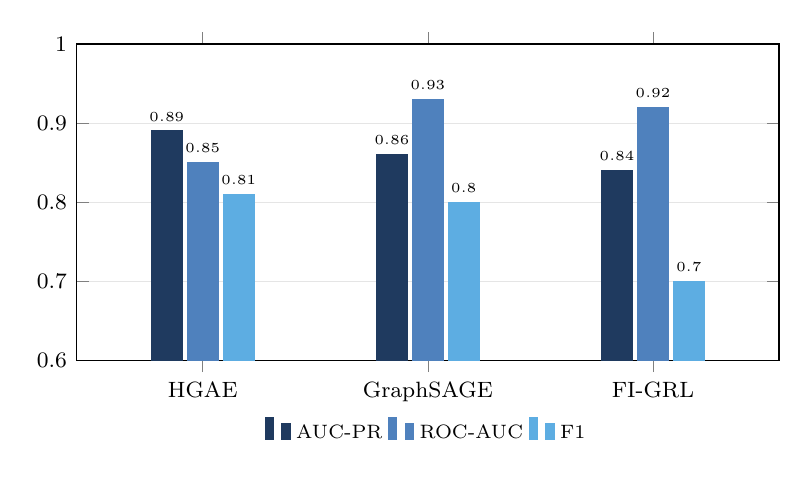
\begin{tikzpicture}
  \begin{axis}[
      ybar,
      width=10.5cm,height=5.6cm,
      ymin=0.6,ymax=1.0,
      bar width=11pt,
      enlarge x limits=0.28,
      ymajorgrids,grid style={gray!20},
      symbolic x coords={HGAE,GraphSAGE,FI-GRL},
      xtick=data,
      ytick={0.6,0.7,0.8,0.9,1.0},
      tick label style={font=\footnotesize},
      legend style={at={(0.5,-0.16)},anchor=north,legend columns=3,font=\scriptsize,draw=none},
      nodes near coords,
      nodes near coords style={font=\tiny},
      every node near coord/.append style={anchor=south}]
    \addplot[draw=mDark,fill=mDark]   coordinates {(HGAE,0.89)(GraphSAGE,0.86)(FI-GRL,0.84)};
    \addplot[draw=mBlue,fill=mBlue]   coordinates {(HGAE,0.85)(GraphSAGE,0.93)(FI-GRL,0.92)};
    \addplot[draw=mAccent,fill=mAccent] coordinates {(HGAE,0.81)(GraphSAGE,0.80)(FI-GRL,0.70)};
    \legend{AUC-PR,ROC-AUC,F1}
  \end{axis}
\end{tikzpicture}
\\[0.2em]
  {\footnotesize \rd{HGAE leads on AUC-PR \& F1 --- but its ROC-AUC is the lowest.}}
\end{frame}
\note{2 min. Orange (AUC-PR): HGAE .89 highest. Blue (ROC-AUC): HGAE .85 LOWEST. Green (F1): .81. Trade-off, not blanket win.}

% ---- Comparison table + verdict ----
\begin{frame}{Comparison --- superiority is nuanced, not uniform}
  \centering
  \begin{tabular}{lccc}
    \arrayrulecolor{mDark}\toprule
    \rowcolor{mDark}\textcolor{white}{\textbf{Method}} & \textcolor{white}{\textbf{AUC-PR}} & \textcolor{white}{\textbf{F1}} & \textcolor{white}{\textbf{ROC-AUC}}\\
    \midrule
    \rowcolor{mBlue!10}\textbf{HGAE} & \ob{0.89} & \ob{0.81} & \rd{0.85}\\
    GraphSAGE & 0.86 & 0.80 & \gr{0.93}\\
    \rowcolor{mBlue!10}FI-GRL & 0.84 & 0.70 & \gr{0.92}\\
    \bottomrule
  \end{tabular}
  \vspace{0.6em}
  \begin{block}{Verdict}
    Wins where it matters under imbalance (\ob{AUC-PR}, \ob{F1}), but \rd{loses on ROC-AUC} --- a trade-off the original paper never reconciles.
  \end{block}
\end{frame}
\note{1.5 min. The paper claims superiority; its own ROC-AUC contradicts a blanket claim. Q: "deal-breaker?" -> depends on operating context.}

% ---- Discussion / formulation critique (still part of Results) ----
\begin{frame}{Discussion --- five formulation concerns}
  \begin{enumerate}\small
    \item \rd{Implausible depth}: 124 layers vs.\ oversmoothing $\rightarrow$ not reproducible
    \item \rd{Attribute-only decoding}: structure enters the score only \emph{indirectly}
    \item \rd{Incomplete VAE}: no KL term $\rightarrow$ weak ``variational'' claim
    \item \rd{Overstated superiority}: lowest ROC-AUC, never reconciled
    \item \rd{Ambiguous threshold}: $\mu+2\sigma$ vs.\ F1-sweep $\rightarrow$ possible leakage
  \end{enumerate}
  \begin{takeaway}
    \#2 is the deepest: it undercuts the paper's own ``topology is what others miss''.
  \end{takeaway}
\end{frame}
\note{2 min. Our original contribution. Internally-consistent criticisms tied to evidence shown earlier.}

% ---- Limitations ----
\begin{frame}{Limitations inherited from the GNN family}
  \begin{columns}[T]
    \begin{column}{0.5\textwidth}
      \begin{itemize}\small
        \item \rd{Scalability}: $O(nE)$ full-graph infeasible
        \item \rd{Static-graph fallacy}: blind to velocity attacks
        \item \rd{Heterophily}: fraud camouflages among legit
      \end{itemize}
    \end{column}
    \begin{column}{0.5\textwidth}
      \begin{itemize}\small
        \item \rd{No explainability}: opaque score
        \item \rd{Oversmoothing / -squashing} with depth
        \item \rd{Latent collapse}: no contrastive term
      \end{itemize}
    \end{column}
  \end{columns}
  \vspace{0.3em}
  {\footnotesize These map back to the \hl{challenges} raised at the start --- the loop closes.}
\end{frame}
\note{2 min. Family-level constraints. Q: "any solved?" -> sampling for scale, temporal GNNs for drift; combined unsupervised still open.}

% =====================================================================
\section{Conclusion}
% =====================================================================
\sectionintro{6}{Conclusion}
  {Key takeaways and a research agenda for robust, label-free fraud detection.}
\note{Bridge: We have seen both the strengths and the cracks --- strong precision/recall, but real formulation and GNN-family limits. To close, we distil the takeaways and lay out concrete future directions, each tied to a limitation.}

% ---- Future work ----
\begin{frame}{Future work --- every fix targets a named limitation}
  \begin{itemize}\small
    \item \hl{Masked \& contrastive GAEs} (MGAE, lrGAE) $\rightarrow$ collapse + attribute-only
    \item \hl{Architectural simplification} (linear prop., orthogonal init) $\rightarrow$ scale + depth
    \item \hl{Temporal heterogeneous GNNs} $\rightarrow$ velocity / evolving fraud
    \item \hl{Adaptive thresholds} $\rightarrow$ drop the global Gaussian assumption
    \item \hl{Explainable attribution} $\rightarrow$ per-attribute loss, attention maps
  \end{itemize}
\end{frame}
\note{2 min. Pair each remedy with its flaw. Q: "first?" -> contrastive masked AE + temporal extension.}

% ---- Conclusion ----
\begin{frame}{Conclusion}
  \begin{itemize}
    \item GAEs reframe fraud as \gr{one-class anomaly detection} --- beating label scarcity
    \item HGAE fuses \hl{type-specific attention} + unsupervised reconstruction
    \item But superiority is \rd{nuanced}; formulation \& GNN limits remain
    \item Forward: \bl{masked/contrastive, temporal, simplified, explainable}
  \end{itemize}
  \begin{takeaway}
    Learn what \emph{normal} looks like on the graph and let fraud betray itself ---
    but verify every claim honestly.
  \end{takeaway}
\end{frame}
\note{1.5 min. Pull the arc together. End on the meta-lesson: restraint + honest evaluation over hype.}

% ---- Closing ----
\begin{frame}[standout]
  \huge{Thank you --- Questions?}

  \vspace{0.8cm}
  \rule{\linewidth}{0.5pt}
  \vspace{0.8cm}

  % \Large{Credit Card Fraud Detection using Graph Auto-Encoder}
\end{frame}

\note{Backup: 124-layer issue, KL absence, AUC-PR vs ROC-AUC, masked/contrastive benefits, dataset provenance, deployment latency, vs Isolation Forest.}

% ---- References ----
\begin{frame}{References}
  \footnotesize
  \begin{enumerate}
    \item Majumder, S., Singh, M.\,T., Prasad, R.\,K., et al.\ \emph{Heterogeneous Graph Auto-Encoder for Credit Card Fraud Detection}. International Journal of Computer Applications (IJCA), 32(2), 124--138, 2025.
    \item Liu, Z., Chen, C., Yang, X., Zhou, J., Li, X., Song, L.\ \emph{Heterogeneous Graph Neural Networks for Malicious Account Detection}. CIKM~'18, 2077--2085, 2018.
    \item Kipf, T.\,N., Welling, M.\ \emph{Variational Graph Auto-Encoders}. arXiv:1611.07308, 2016.
    \item Alon, U., Yahav, E.\ \emph{On the Bottleneck of Graph Neural Networks and its Practical Implications}. ICLR, 2021.
    \item Emergent Mind.\ \emph{Graph Neural Network (GNN)-based Autoencoders}. Online resource, \url{https://www.emergentmind.com}, 2026 (updated Jan 2026).
  \end{enumerate}
\end{frame}


\end{document}

\end{document}
